\chapter{基于深度相机模型形变捕捉}
要构建模型的形变子空间,除了静态三维模型,
还需要一些形变后的模型,即形变关键帧作为输入。
本章描述了一个以静态模型和深度视频为输入的形变捕捉算法。
在捕捉步骤中,操作者会带着特定颜色的手套,在深度相机前摆弄物体,使得物体发生形变。
该算法会优化模型的形变参数,使得模型的形状和相机采集的物体形状尽量吻合,
从而得到形变后的模型。
本文会从捕捉到的形变中选取若干成为形变关键帧,作为形变子空间构建的输入。
本章接下来就会阐述该算法的技术细节。

\section{基于手部信息的模型初始位姿估计}

 类似于三维重建步骤中的相机位姿估计,
 在形变步骤中,对于每一帧深度图像,本文仅计算模型和上一帧的相对形变。
 因此,在捕捉形变之前,需要得知模型的初始位置。
 在本文的形变捕捉流程中,操作者需要用手持物。
 所以物体必然位于手的附近,所以本文设计了一个借助手部信息确定模型的初始位置与朝向的算法。
 本位所采用的确定物体初始位姿的算法可主要分为三个步骤:分割手部点云、分割物体点云、模型对齐。
 本节接下来就会详细描述这一流程。

\subsection{手部点云分割}
由于本文是借助手部点云的位置寻找物体的点云,
所以需要在输入的点云中分割出属于手的部分。
本章就将描述一种基于RGBD图像的点云分割算法。
\begin{figure}[h]
    \centering
    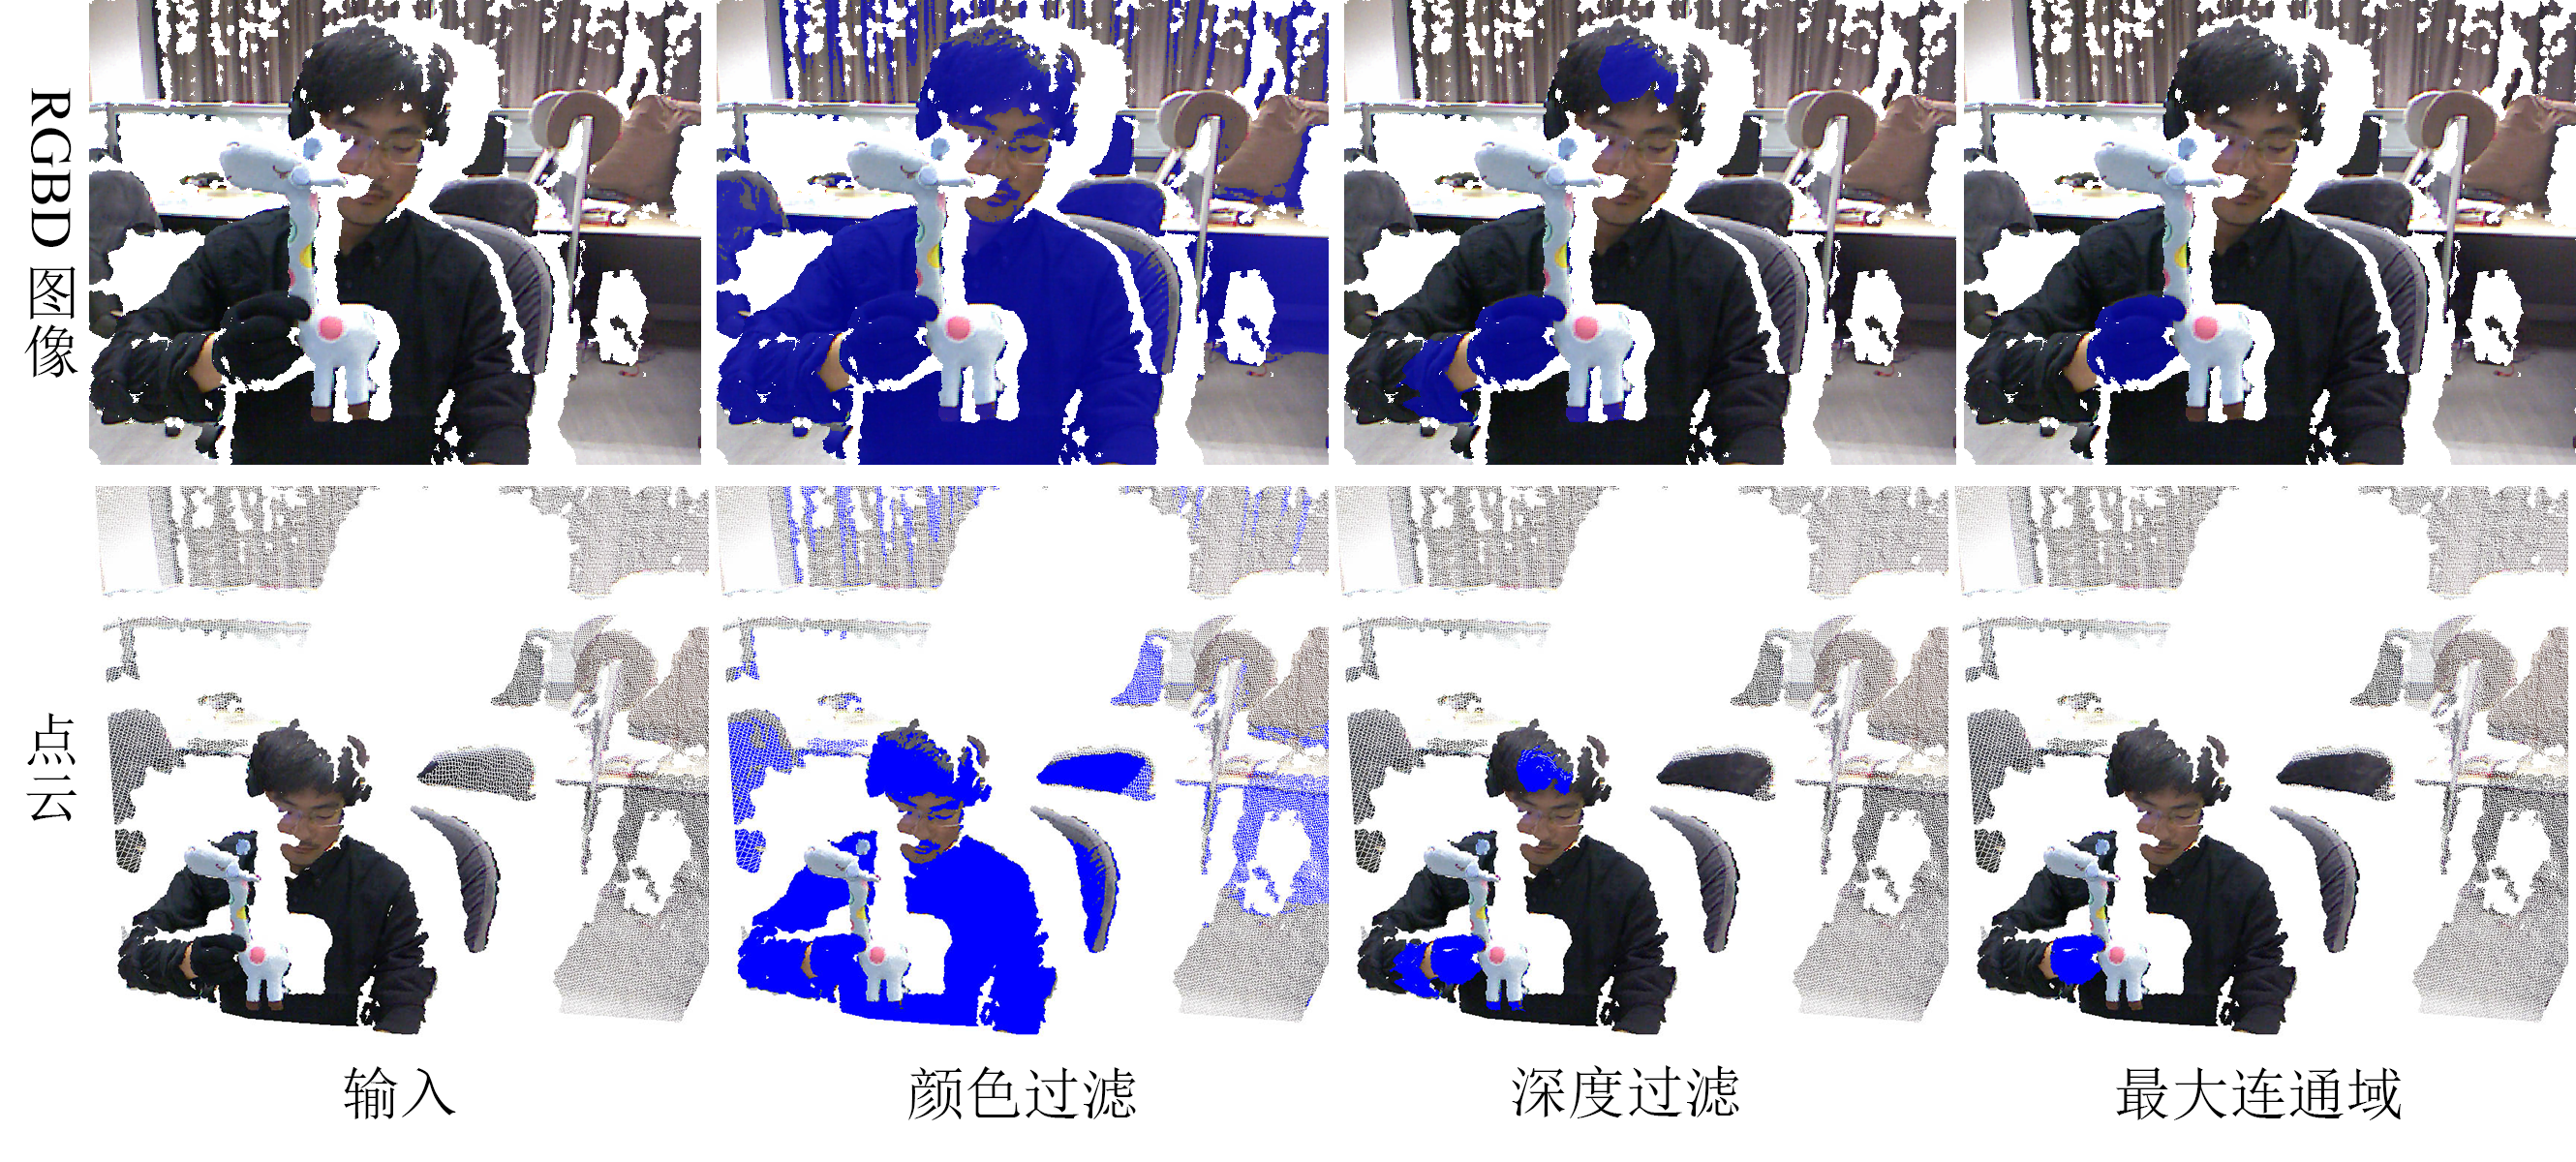
\includegraphics[width = \textwidth]{./Pictures/FindingHand.png}
    \caption{手部点云分割流程}
    \label{finding_hand}
\end{figure}
分割手部点云阶段的输入是RGBD图像,输出为手部的像素坐标的集合。
RGBD图像即除了RGB三个颜色通道外,还有一个深度通道
记录了对应点距离相机的距离,可以理解为RGB图像加上深度图像。
Kinect分别通过色彩传感器和深度传感器获得RGB图像和深度图像,
由于两个传感器的相对位置被事先标定过,
所以Kinect的SDK提供了将RGB图像映射到深度图像的接口,
映射后的RGB图像的像素和深度图像的像素一一对应。
图\ref{finding_hand}第一行的第一张图就是映射到相应深度图位置后的RGB图像。
本文中提到的RGB图像均默认指映射后的RGB图像。

在操作物体时,操作者会带上特定颜色的手套,以对相应的数据做特殊处理。
找出手部数据的主要目的是在后续的形变捕捉步骤中过滤掉所有手部的深度信息,
因为手部的深度信息对于形变捕捉是很大的噪声。
在形变捕捉的前置阶段——初始位置阶段,
手部信息也作为辅助信息用于确定物体的初始位姿
如图\ref{finding_hand}和算法\ref{alg_seg_hand}所示,
分割手部点云阶段可主要分为颜色过滤、深度过滤、寻找最大连通域三个步骤。
图\ref{finding_hand}的第一行的图片中被标记为蓝色的部分是每个步骤确定的手的位置,
第二行的图片是对应的点云。
\begin{algorithm}
    \fangsong
    \caption{分割手部点云}
    \label{alg_seg_hand}
    \begin{algorithmic}[1]
        \Require RGB图像$\mathbf{C_i}$,深度图像$\mathbf{D_i}$
        \Ensure 手部像素集合$\mathbf{S_{hand}}$
        \Procedure{GetHandPixels}{$\mathbf{C_i}$, $\mathbf{D_i}$}
            %\State $\mathbf{V_i} \gets$ \Call{DepthToVertex}{$\mathbf{D_i}$}
            \State $\mathbf{S_{hand}} \gets$ \Call{ColorFilter}{$\mathbf{C_i}$}
            \State $\mathbf{S_{hand}} \gets$ \Call{DepthFilter}{$\mathbf{D_i}$, $\mathbf{S_{hand}}$}
            \State $\mathbf{S_{hand}} \gets$ \Call{LargestConnectedDomain}{$\mathbf{S_{hand}}$}
        \EndProcedure
    \end{algorithmic}
\end{algorithm}

首先,本文会进行颜色过滤步骤,筛选出输入图像中与手套颜色相近的像素点。
算法\ref{alg_cfilter}描述了颜色过滤的流程。
其中$\mathbf{C_{hand}}$和$thd_{color}$分别是预先设定的手套颜色的集合和颜色距离阈值。
%本文的实验中$thd_{color}$的值设为50。
在该步骤中,会遍RGB图像的每一个像素。
如果该像素的颜色和$\mathbf{C_{hand}}$中的任何颜色相近,
即在RGB颜色空间中与相应颜色距离小于$thd_{color}$的像素,
就会被认为可能是手部的像素,并入待选集合中。
颜色过滤的记过如图\ref{finding_hand}中第二列所示。
从图中可以看出,颜色过滤会将图像背景中大量颜色与手套相近的像素判定为手部像素。
所以,如果要借助手的位置确定物体的位置,还需要进一步的筛除背景中多余的像素。
\begin{algorithm}
    \fangsong
    \caption{颜色过滤}
    \label{alg_cfilter}
    \begin{algorithmic}[1]
        \Require RGB图像$\mathbf{C_i}$
        \Ensure 像素点集合$\mathbf{S}$
        \Function {ColorFilter}{$\mathbf{C_i}$}
            %\State $\mathbf{S} \gets \varnothing$
            \For {$\forall\mathbf{u} \in$ \Call{PixelDomain}{$\mathbf{C_i}$}}
                \For {$\forall\mathbf{c} \in \mathbf{C_{hand}}$}
                    \If{$\|\mathbf{C_i}(u) - \mathbf{c}\| \leq thd_{color}$}
                    \State $\mathbf{S} \gets \mathbf{S} \bigcup \{\mathbf{c}\}$
                    \EndIf
                \EndFor
            \EndFor 
            \State \Return $\mathbf{S}$
        \EndFunction
    \end{algorithmic}
\end{algorithm}

在颜色过滤后,本文会执行深度过滤步骤,即只保留深度最小像素点。
从图\ref{finding_hand}中可以看出,在操作者手持物体操作的过程中,
握着物体的手总是位于最前方。
%在这种特定的场景中,本文默认手部的像素点必在深度值最小的那部分像素之中。
算法\ref{alg_dfilter}描述了深度过滤的流程。
其中,$d_{range}$是预先设定的筛选深度范围,%在本文的实验中设为150毫米。
$d_{min}$是集合中深度最小的像素的深度值。
然后遍历集合中的每个像素,仅保留深度值小于$d_{min}+d_{range}$的像素。
深度过滤的结果如图\ref{finding_hand}第三列所示。
% \begin{algorithm}
%     \fangsong
%     \caption{深度图像转点云}
%     \label{alg_d2v}
%     \begin{algorithmic}
%         \Require 深度图像$\mathbf{D_i}$
%         \Ensure 点云$\mathbf{V_i}$
%         \Function {DepthToVertex}{$D_i$}
%             \For{$\forall \mathbf{u} \in$ \Call{PixelDomain}{$\mathbf{D_i}$}}
%                 \State $\mathbf{V_i(u)}=\mathbf{D_i}(\mathbf{u})\mathbf{K}^-1[\mathbf{u},1]$
%             \EndFor
%             \State \Return $\mathbf{V_i}$
%         \EndFunction
%     \end{algorithmic}
% \end{algorithm}
\begin{algorithm}
    \fangsong
    \caption{深度过滤}
    \label{alg_dfilter}
    \begin{algorithmic}[1]
        \Require 深度图像$\mathbf{D_i}$, 像素点集合$\mathbf{S_{in}}$
        \Ensure 像素点集合$\mathbf{S_{out}}$
        \Function {DepthFilter}{$\mathbf{D_i}$, $\mathbf{S_{in}}$}
            %\State $\mathbf{Set_{out}} \gets \mathbf{Set_{int}}$
            \State $d_{min} \gets$ \Call{Min}{$\mathbf{D_i}$}
            \For {$\forall \mathbf{u} \in \mathbf{S_{in}}$}
                \If {$\mathbf{D_i}(\mathbf{u}) < d_{min}$ or $\mathbf{D_i}(\mathbf{u}) > d_{min} + d_{range}$}
                    %\State $\mathbf{Set_out} \gets \mathbf{S} - \{u\}$
                    \State $\mathbf{S_{out}} \gets \mathbf{S_{out}} \bigcup \{\mathbf{u}\}$
                \EndIf
            \EndFor
            \State \Return $\mathbf{S_{out}}$
        \EndFunction
    \end{algorithmic}
\end{algorithm}
\begin{algorithm}
    \fangsong
    \caption{获取最大连通域}
    \label{alg_lcd}
    \begin{algorithmic}[1]
        \Require 像素点集合$\mathbf{S}$
        \Ensure 最大连通域$\mathbf{LCD}$
        \Function {LargestConnectedDomain}{$\mathbf{S}$}
            %\State $\mathbf{LCD} \gets \varnothing$
            \For{$\forall \mathbf{u} \in \mathbf{S}$}
                \If{$\mathbf{u}$ not checked}
                    \State $\mathbf{CD} \gets$ \Call{GetConnectedDomain}{$\mathbf{S}$, $\mathbf{u}$}
                    \If{$|\mathbf{CD}| > |\mathbf{LCD}|$}
                        \State $\mathbf{LCD} \gets  \mathbf{CD}$
                    \EndIf
                \EndIf
            \EndFor
            \State \Return $\mathbf{LCD}$
        \EndFunction
        \Function {GetConnectedDomain}{$\mathbf{S}$, $\mathbf{u}$}
            %\State $Q \gets$ \Call{EmptyQueue}{},$\mathbf{CD} \gets \varnothing$
            \State \Call{QueuePush}{$Q$, $\mathbf{u}$}
            \State Set $\mathbf{u}$ as checked
            \While{$Q$ not empty}
                \State $\mathbf{u_i} \gets$ \Call{QueuePop}{$Q$}
                \State $\mathbf{CD} \gets \mathbf{CD} \bigcup \{\mathbf{u_i}\}$
                \For{$\forall \mathbf{u_{neighbor}} \in$ \Call{NeighborPixel}{$\mathbf{u_i}$}}
                    \If{$\mathbf{u_{neighbor}}$ not checked}
                        \State \Call{QueuePush}{$Q$, $\mathbf{u_{neighbor}}$}
                        \State Set $\mathbf{u_{neighbor}}$ as checked
                    \EndIf
                \EndFor
            \EndWhile
            \State \Return $\mathbf{CD}$
        \EndFunction
    \end{algorithmic}
\end{algorithm}
在深度过滤后,本文将在已经判定为手部的像素集合中找到其在图像空间中最大连通域,
进一步去除零散的像素点。
以带黑色手套为例,这些被误判的像素点可能是物体上阴影所在的部分,
也可能是身体靠近物体的部分。
这些被误判的区域会影响物体位置的估计。
在实验的过程中可以发现,在深度过滤之后,真正的手部在图像中,
大都落在已判定区域中的最大连通域里。
所以本文在深度过滤的结果中寻找图像空间中的最大连通域,作为最终的手部区域。
算法\ref{alg_lcd}描述了该步骤的流程。
GetConnectedDomain函数采用了广度优先搜索的方式计算与指定像素位置$\mathbf{u}$
相连的连通域;
LargestConnectedDomain函数遍历了集合中所有的连通域,并找到其中最大的连通域。
最终分割出的手部点云如图\ref{finding_hand}第四列所示。

在上述步骤中,颜色过滤和深度过滤各像素位置的计算是互相独立的,可用GPU并行加速。
其中颜色过滤在实现时与RGB图映射到深度图的步骤在同一个CUDA Kernel中实现。
最大连通域的计算需要根据各像素的邻接关系,不便于大规模并行。
且经由之前的筛选,该步骤需要遍历的像素已大为减少,所以在CPU上可以很快的完成。


\subsection{物体点云分割}

\subsection{模型对齐}

\section{基于深度视频的形变捕捉}
\subsection{形变的参数化描述}
\subsection{形变参数优化}

\section{本章小结}